\chapter{قالب لاتک برای پایان‌نامه}
فایل‌های حاضر جهت حروف‌چینی پایان‌نامه‌ها در نرم‌افزار لاتک (در دانشکده‌های فنی دانشگاه تهران) تهیه شده‌اند. نرم‌افزار لاتک
\LTRfootnote{Latex}
یک نرم‌افزار حروف‌چینی رایگان است که تحت سیستم عامل‌های مختلف قابل استفاده می‌باشد. با افزودن بسته زی‌پرشین
\LTRfootnote{XePersian}
امکان حروف‌چینی فارسی با تمام فونت‌های فارسی نصب شده روی سیستم عامل با نرم‌افزار لاتک فراهم گردید. این قالب با استفاده از مطالب سایت پارسی لاتک
\LTRfootnote{http://parsilatex.com/site}
تهیه شده است. در این سایت مطالب آموزشی مختلف در خصوص لاتک و بسته زی‌پرشین وجود دارد.

\section{توضیح فایل‌ها}
فایل اصلی این قالب فایل thesis.tex است. جهت تولید فایل صحفح آرایی شده این فایل باید کامپایل شود. تنظیمات کلی نظیر فونت و بسته‌های لازم در فایل header.tex قرار گرفته‌اند. در این فایل تنظیمات حداقلی قرار داده شده‌اند. برای مثال فونت این متن \lr{XB~Zar} می‌باشد. برای کامپایل صحیح این فونت باید روی سیستم شما نصب باشد. در غیر این صورت فونت فوق را نصب نمایید یا آن را با یک فونت نصب شده جایگزین کنید. دانشجویان با توجه به موضوع و زمینه پژوهشی خود می‌توانند تنظیمات و بسته‌های بیشتری به این فایل بیفزایند. برای مثال برای کُدنویسی بسته listings و یا برای حروف‌چینی معادلات شیمیایی بسته mhchem بسیار مفید هستند.

صفحات اول پایان‌نامه در پوشه First-Pages قرار دارند. محتویات فایل‌های درون پوشه با توجه به مشخصات پایان‌نامه باید اصلاح شوند. برای گواهی دفاع از پایان‌نامه، اصل گواهی در نسخه چاپی جایگزین شود یا یک اسکن با کیفیت تهیه و جایگزین فایل Govahi.jpg در پوشه فوق گردد.

توصیه می‌شود هر فصل پایان‌نامه در یک فایل جدا نوشته شود. برای مثال فصل‌های این متن به صورت chapter1.tex ، chapter2.tex و ... تهیه شده‌اند.

\section{روابط ریاضی}
از جمله قابلیت‌های مهم لاتک حروف‌چینی روابط ریاضی است. در ادامه نمونه‌هایی از روابط ریاضی مختلف نشان داده می‌شود:
\begin{equation}
y = f(x) = \sin x + e^x + \sqrt{1+x^2} - \frac{\sqrt[3]{1+x^3}}{1+x}
\end{equation}
\begin{eqnarray}
&&\vec{F} = m \vec{a} = m \frac{d^2\vec{r}}{dt^2} \\
&&\vec{F} = (F_x,F_y,F_z), \quad \vec{r} = (x,y,z) \nonumber
\end{eqnarray}
\begin{eqnarray}
\lim_{x\rightarrow p} f(x) = L \quad \Leftrightarrow \quad 
\forall \epsilon > 0  \;\; \exists \delta>0 \;\mid\; \forall x \in [p-\delta,p+\delta] \Rightarrow |f(x)-L|<\epsilon
\end{eqnarray}
\begin{eqnarray}
A\cap (B\cup C ) = (A\cap B)\cup (A\cap C )
\end{eqnarray}
\begin{eqnarray}
G_{\mu\nu} = \frac{8\pi G}{c^4}T_{\mu\nu} , \qquad G_{\mu\nu} \equiv R_{\mu\nu}-\frac{1}{2}Rg_{\mu\nu}
\end{eqnarray}
\begin{eqnarray}
\nabla^2 \phi = \frac{\partial^2 \phi}{\partial x^2}+
\frac{\partial^2 \phi}{\partial y^2}+
\frac{\partial^2 \phi}{\partial z^2}
\end{eqnarray}
\begin{eqnarray}
\hat{f}(\omega)=&\mathcal{F}(f)(\omega) &= \int_{-\infty}^{\infty} f(x) e^{-2\pi i \omega x} \;dx \\
f(x)=&\mathcal{F}^{-1}(\hat{f})(x) &= \int_{-\infty}^{\infty} \hat{f}(\omega) e^{2\pi i x \omega } \;d\omega
\end{eqnarray}

\section{جدول‌ها}
جدول‌ها برای ارائه داده‌ها و نتايج بسیار استفاده می‌شوند. جدول‌های \ref{tab-1} و \ref{tab-2} نمونه‌ای از یک جدول فارسی و انگلیسی را نشان می‌دهند. به طور پیش‌فرض با استفاده از بسته زی‌پرشین جدول‌ها راست‌چین هستند. شماره و توضیح هر جدول باید در بالای آن قرار داشته باشد. 

\begin{table}[h]
\caption{مثالی از یک جدول فارسی}
\centering
\begin{tabular}{|r|r|} \hline\hline
نام روش & زمان (ms) \\ \hline\hline
روش مرتبه دوم  & 105.42  \\
روش مرتبه چهارم & 213.03 \\\hline
\end{tabular}
\label{tab-1}
\end{table}

\begin{table}[h]
\latin
\caption{An example of a table in English}
\centering
\begin{tabular}{|l|l|} \hline\hline
Scheme & time (ms) \\ \hline\hline
second-order method & 105.42 \\
fourth-order method & 213.03\\\hline
\end{tabular}
\label{tab-2}
\end{table}


\section{شکل‌ها}
بخشی از داده‌ها و نتایج با استفاده از شکل‌ها ارائه می‌گردند. شکل‌ها می‌توانند شامل نمودار، عکس، دیاگرام یا ... باشند. روش‌های مختلفی برای تولید شکل وجود دارند. حتی با استفاده از برخی دستورات و بسته‌های لاتک می‌توان شکل‌های مورد نظر را تولید نمود. با این حال معمولاً شکل‌ها در قالب یک عکس با نرم‌افزارهای مختلف تولید و در پایان‌نامه ارائه می‌شوند.
توصیه می‌گردد برای تصاویر واقعی یا نتایجی که در آن تمام مساحت عکس رنگی است از فرمت‌های نظیر jpg جهت ذخیره‌سازی استفاده شود (شکل \ref{fig.1}). برای نمودارها بهتر است از فرمت‌های ذخیره‌سازی برداری نظیر eps استفاده شود (شکل \ref{fig.2}). فرمت‌های برداری شکل‌های بسیار با کیفیتی هم در نسخه الکترونیکی و هم در نسخه چاپی ایجاد می‌کنند. بیشتر نرم‌افزارهای داده‌برداری آزمایشگاهی و نیز نرم‌افزارهای شبیه‌سازی امکان تولید تصویر با انواع فرمت‌ها را دارا می‌باشند. شماره و توضیح هر شکل باید در پایین آن قرار داشته باشد. 

\begin{figure}[h]\centering
\includegraphics[width=\textwidth]{Figures/contour.jpg}
\caption{%
نمونه یک شکل با فرمت \lr{jpg}
}
\label{fig.1}
\end{figure}

\begin{figure}[h]\centering
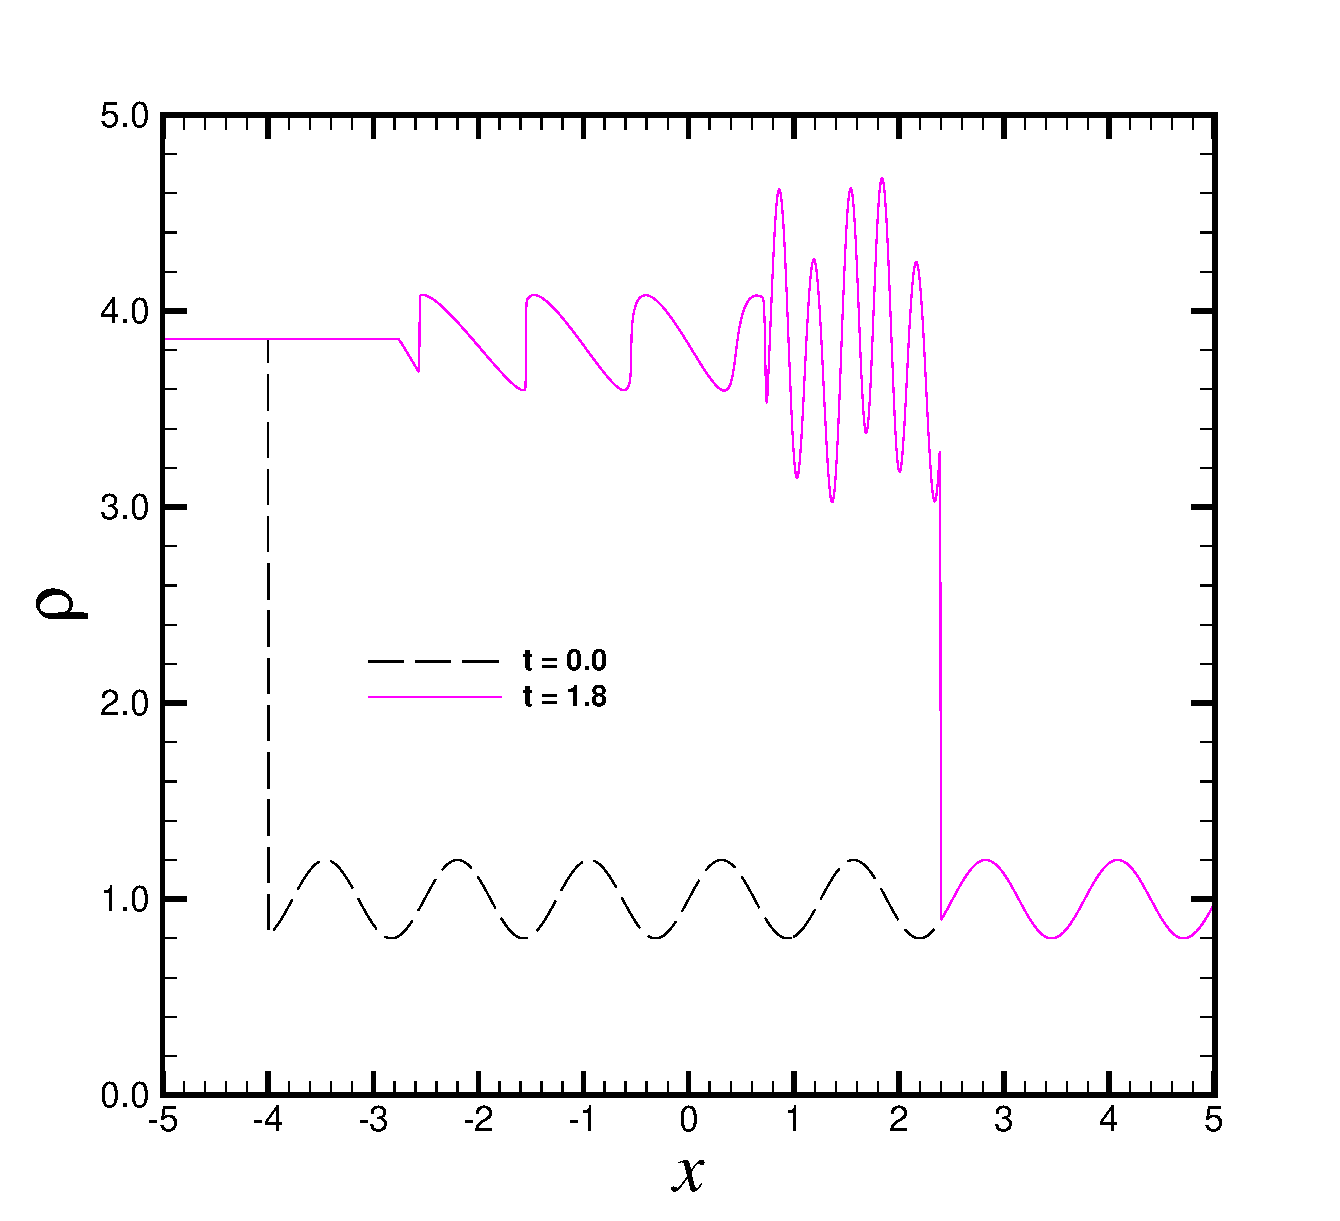
\includegraphics[width=0.7\textwidth]{Figures/density.eps}
\caption{%
نمونه یک شکل با فرمت \lr{eps} که به صورت برداری ذخیره شده است.
}
\label{fig.2}
\end{figure}


